\documentclass[]{article}
\usepackage{lmodern}
\usepackage{amssymb,amsmath}
\usepackage{ifxetex,ifluatex}
\usepackage{fixltx2e} % provides \textsubscript
\ifnum 0\ifxetex 1\fi\ifluatex 1\fi=0 % if pdftex
  \usepackage[T1]{fontenc}
  \usepackage[utf8]{inputenc}
\else % if luatex or xelatex
  \ifxetex
    \usepackage{mathspec}
  \else
    \usepackage{fontspec}
  \fi
  \defaultfontfeatures{Ligatures=TeX,Scale=MatchLowercase}
\fi
% use upquote if available, for straight quotes in verbatim environments
\IfFileExists{upquote.sty}{\usepackage{upquote}}{}
% use microtype if available
\IfFileExists{microtype.sty}{%
\usepackage{microtype}
\UseMicrotypeSet[protrusion]{basicmath} % disable protrusion for tt fonts
}{}
\usepackage[margin=1in]{geometry}
\usepackage{hyperref}
\hypersetup{unicode=true,
            pdftitle={Analysis of excess influenza-like illness during the novel corona virus (2020) outbreak},
            pdfauthor={Nicholas G Reich, Caitlin Rivers},
            pdfborder={0 0 0},
            breaklinks=true}
\urlstyle{same}  % don't use monospace font for urls
\usepackage{graphicx,grffile}
\makeatletter
\def\maxwidth{\ifdim\Gin@nat@width>\linewidth\linewidth\else\Gin@nat@width\fi}
\def\maxheight{\ifdim\Gin@nat@height>\textheight\textheight\else\Gin@nat@height\fi}
\makeatother
% Scale images if necessary, so that they will not overflow the page
% margins by default, and it is still possible to overwrite the defaults
% using explicit options in \includegraphics[width, height, ...]{}
\setkeys{Gin}{width=\maxwidth,height=\maxheight,keepaspectratio}
\IfFileExists{parskip.sty}{%
\usepackage{parskip}
}{% else
\setlength{\parindent}{0pt}
\setlength{\parskip}{6pt plus 2pt minus 1pt}
}
\setlength{\emergencystretch}{3em}  % prevent overfull lines
\providecommand{\tightlist}{%
  \setlength{\itemsep}{0pt}\setlength{\parskip}{0pt}}
\setcounter{secnumdepth}{0}
% Redefines (sub)paragraphs to behave more like sections
\ifx\paragraph\undefined\else
\let\oldparagraph\paragraph
\renewcommand{\paragraph}[1]{\oldparagraph{#1}\mbox{}}
\fi
\ifx\subparagraph\undefined\else
\let\oldsubparagraph\subparagraph
\renewcommand{\subparagraph}[1]{\oldsubparagraph{#1}\mbox{}}
\fi

%%% Use protect on footnotes to avoid problems with footnotes in titles
\let\rmarkdownfootnote\footnote%
\def\footnote{\protect\rmarkdownfootnote}

%%% Change title format to be more compact
\usepackage{titling}

% Create subtitle command for use in maketitle
\providecommand{\subtitle}[1]{
  \posttitle{
    \begin{center}\large#1\end{center}
    }
}

\setlength{\droptitle}{-2em}

  \title{Analysis of excess influenza-like illness during the novel corona virus
(2020) outbreak}
    \pretitle{\vspace{\droptitle}\centering\huge}
  \posttitle{\par}
    \author{Nicholas G Reich, Caitlin Rivers}
    \preauthor{\centering\large\emph}
  \postauthor{\par}
      \predate{\centering\large\emph}
  \postdate{\par}
    \date{2020-01-24 15:20:07 CET}


\begin{document}
\maketitle

\hypertarget{introduction}{%
\subsection{Introduction}\label{introduction}}

From Caitlin: Is there any chance that what we are observing this year
with our bad flu season is actually nCoV? Is the delta between ILI and
flu positives what you would expect? Is there more than usual wILI that
could be attributable to more widely spread nCoV?

\hypertarget{methods}{%
\subsection{Methods}\label{methods}}

We downloaded publicly available ILINet and WHO-NREVSS data for the
national level and HHS Region 10. HHS Region 10 is the northwest of the
US, where ILI has shown abnormally high levels this season and contains
Washington state, where the initial case of nCoV was detected in the US.
From the ILINet dataset, we downloaded the measure of weighted
influenza-like illness (wILI), which measures, on a weekly scale, the
percentage of doctor's office visits at sentinel providers had the
primary complaint of fever plus an additional influenza-like symptom
(cough, sore throat, etc..). For the WHO-NREVSS data, we obtained the
total number of specimens tested by participating clinical laboratories,
as well as the percent of those speciments that tested positive for
influenza. These data has been aggregated into a single reporting system
since the 2015/2016 season, so we use data since that time. Both data
sources are available at the weekly time-scale, defined as using the
MMWR week standard used by the CDC.

As a first approximation to compute a metric of similarity between the
two metrics, we chose to divide the percent positivity from NREVSS by
the wILI. The resulting ratio should be smaller when wILI values are
high relative to the percent positivity of clinical tests. Therefore,
low values of this metric would indicate that there is lower percent
positivity than ``expected'' given the current levels of wILI. We note
that a limitation of this metric is that wILI values can be quite small,
which could lead to unstable estimates, since this number is in the
denominator.

The code used to produce this report is available on GitHub at
\url{https://github.com/reichlab/ncov}.

\hypertarget{results}{%
\subsection{Results}\label{results}}

We plot three panels for each region considered (national level and HHS
Region 10). We do not detect strong signal of anomalous patterns between
ILI rates and percent positivity with lab data. At the National level
the current season looks similar to past seasons (Figure
\ref{fig:national-plot}). In recent weeks in region 10, the ratio
defined above is smaller than it has been in the past 5 years, although
qualitatively it does not appear to be substantially lower than previous
years (Figure \ref{fig:region10-plot}).

\begin{figure}
\centering
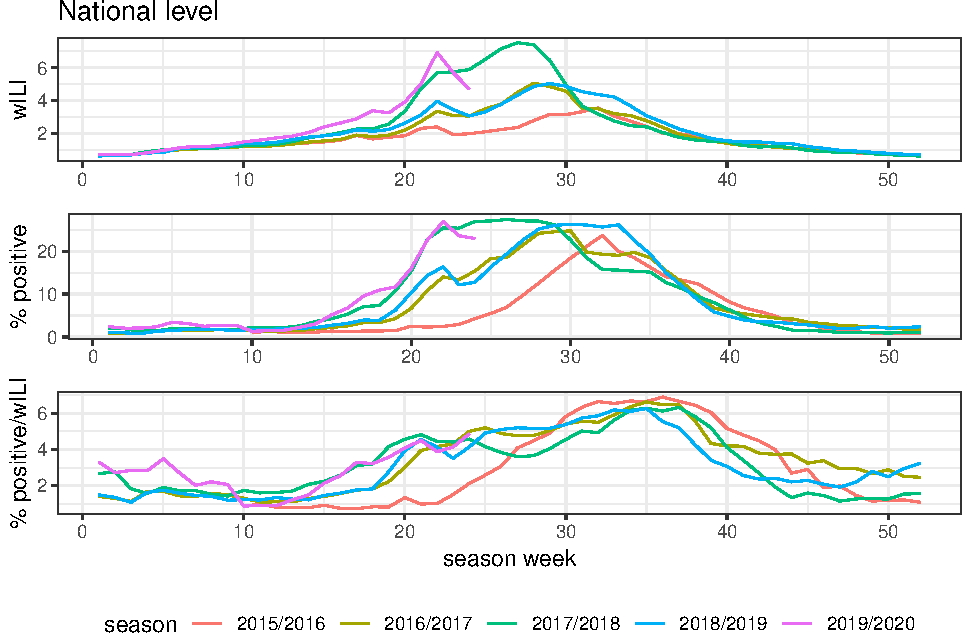
\includegraphics{ili-labtest-report_files/figure-latex/national-plot-1.pdf}
\caption{\label{fig:national-plot}National level plots showing wILI
values since the 2015/2016 season (top), percent of all specimens tested
that are positive for flu (middle), and the ratio of the two (bottom, \%
pos / wILI).}
\end{figure}

\begin{figure}
\centering
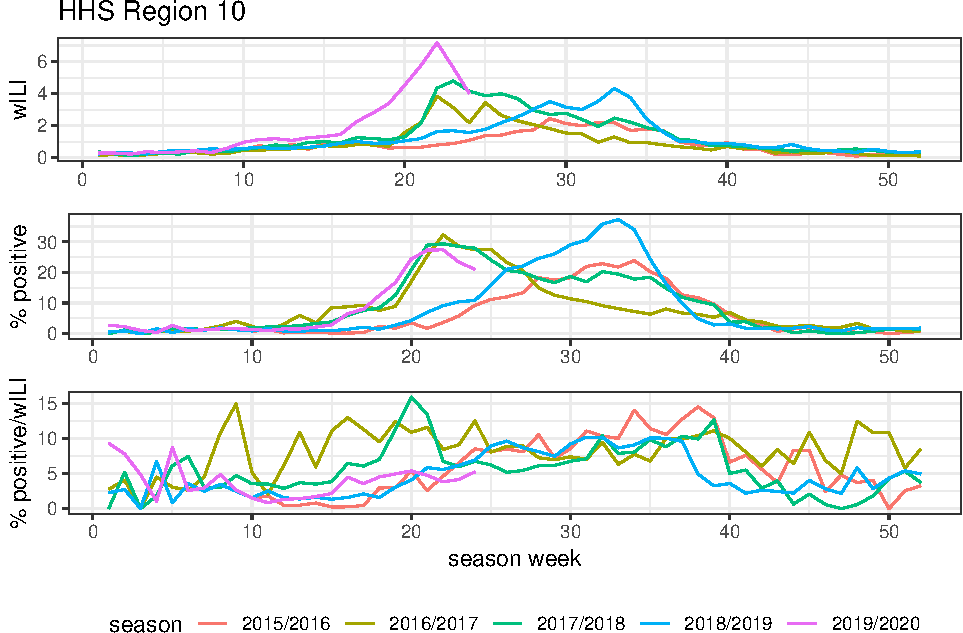
\includegraphics{ili-labtest-report_files/figure-latex/region10-plot-1.pdf}
\caption{\label{fig:region10-plot}US HHS Region 10 plots showing wILI
values since the 2015/2016 season (top), percent of all specimens tested
that are positive for flu (middle), and the ratio of the two (bottom, \%
pos / wILI).}
\end{figure}


\end{document}
